\documentclass{book}
\title{Esercizi di fisica 2 con risoluzione}
\author{Lancillotto dal lago}
\date{\today}

\usepackage[utf8]{inputenc}
\usepackage{enumerate}
\usepackage{amsmath}
\usepackage{mathtools}
\usepackage{graphicx}
% \usepackage{cancel}
\usepackage[right=1.5cm, left=1.5cm]{geometry}

\graphicspath{ {./} }



\begin{document}
\pagenumbering{gobble}
\maketitle



  
%----------------------------------------------------
\chapter{Forza elettrostatica e campo elettrostatico}

\begin{enumerate}
    
    %1.1
    \item Due protoni in un nucleo di elio (He$_2$) distano $d=10^-15m$. Calcolare la forza $f$ con cui interagiscono.\newline
    \textbf{Risoluzione}: data la carica del protone $e = 1,602 \cdot 10^-19 C$ e la distanza $d$ usando la legge di Coulomb si ottiene
    \begin{flalign*}
        F &= \frac{1}{4 \pi \epsilon_0}\frac{q_{1}q_{2}}{d^2}
    \end{flalign*}	
    
    %1.2
    \item Due sferette cariche $q_1$ e $q_2$ si respingono con una forza $F_1 = 5.4 \cdot 10^{–2} N$ quando distano $r = 10 cm$. Sapendo che la loro somma è $q_1 + q_2 = 5 \cdot 10^{–7} C$, calcolare $q_1$ e $q_2$. 
    \newline
    \textbf{Risoluzione}: Con i dati del problema si può facilmente ottenere il prodotto $q_1 \cdot q_2$.
    \begin{align*}
        & F = \frac{1}{4 \pi \epsilon_0}\frac{q_{1}q_{2}}{d^2} \Rightarrow q_1q_2 = F \cdot d^2 \cdot 4 \pi \epsilon_0 = 6 \cdot 10^{-14} 
    \end{align*}
    quindi metteremo a sistema il prodotto fra le due cariche e la loro somma ottenendo così
    \begin{align*}
        \begin{cases}
            q_1 \cdot q_2 = 6 \cdot 10^{-14} \\
            q_1 + q_2 = 5 \cdot 10^{–7}
        \end{cases}
        \begin{cases}
            q_1 = \frac{6 \cdot 10^{-14} }{q_2} \\
            q_2 = 5 \cdot 10^{–7} - \frac{6 \cdot 10^{-14} }{q_2}
        \end{cases}
    \end{align*}
    Ottengo così un polinomio di secondo grado da risolvere
    \begin{align*}
        &\begin{cases}
            q_1 \cdot q_2 = 6 \cdot 10^{-14}  \\
            q_2^2 - 5 \cdot 10^{–7} q_2 + 6 \cdot 10^{-14} = 0
        \end{cases}
        & q_2 = \frac{5 \cdot 10^{-7} \pm \sqrt{(5 \cdot 10^{-7})^2 - 4 \cdot 6 \cdot 10^{-14} }}{2 \cdot 1}
    \end{align*}
    Dunque risolvendo il sistema ottengo
    \begin{align*}
        &\begin{cases}
            q_1 = 3 \cdot 10^{-7} \\
            q_2 = 2 \cdot 10^{-7}
        \end{cases}
    \end{align*}
    
    %1.3
    \item Le due cariche $q_s$ e $q_d$ di ugual carica $q = 2 \cdot 10^{–8} C$ sono poste a distanza $2a = 5 cm$ come in figura.
    \begin{align*}
        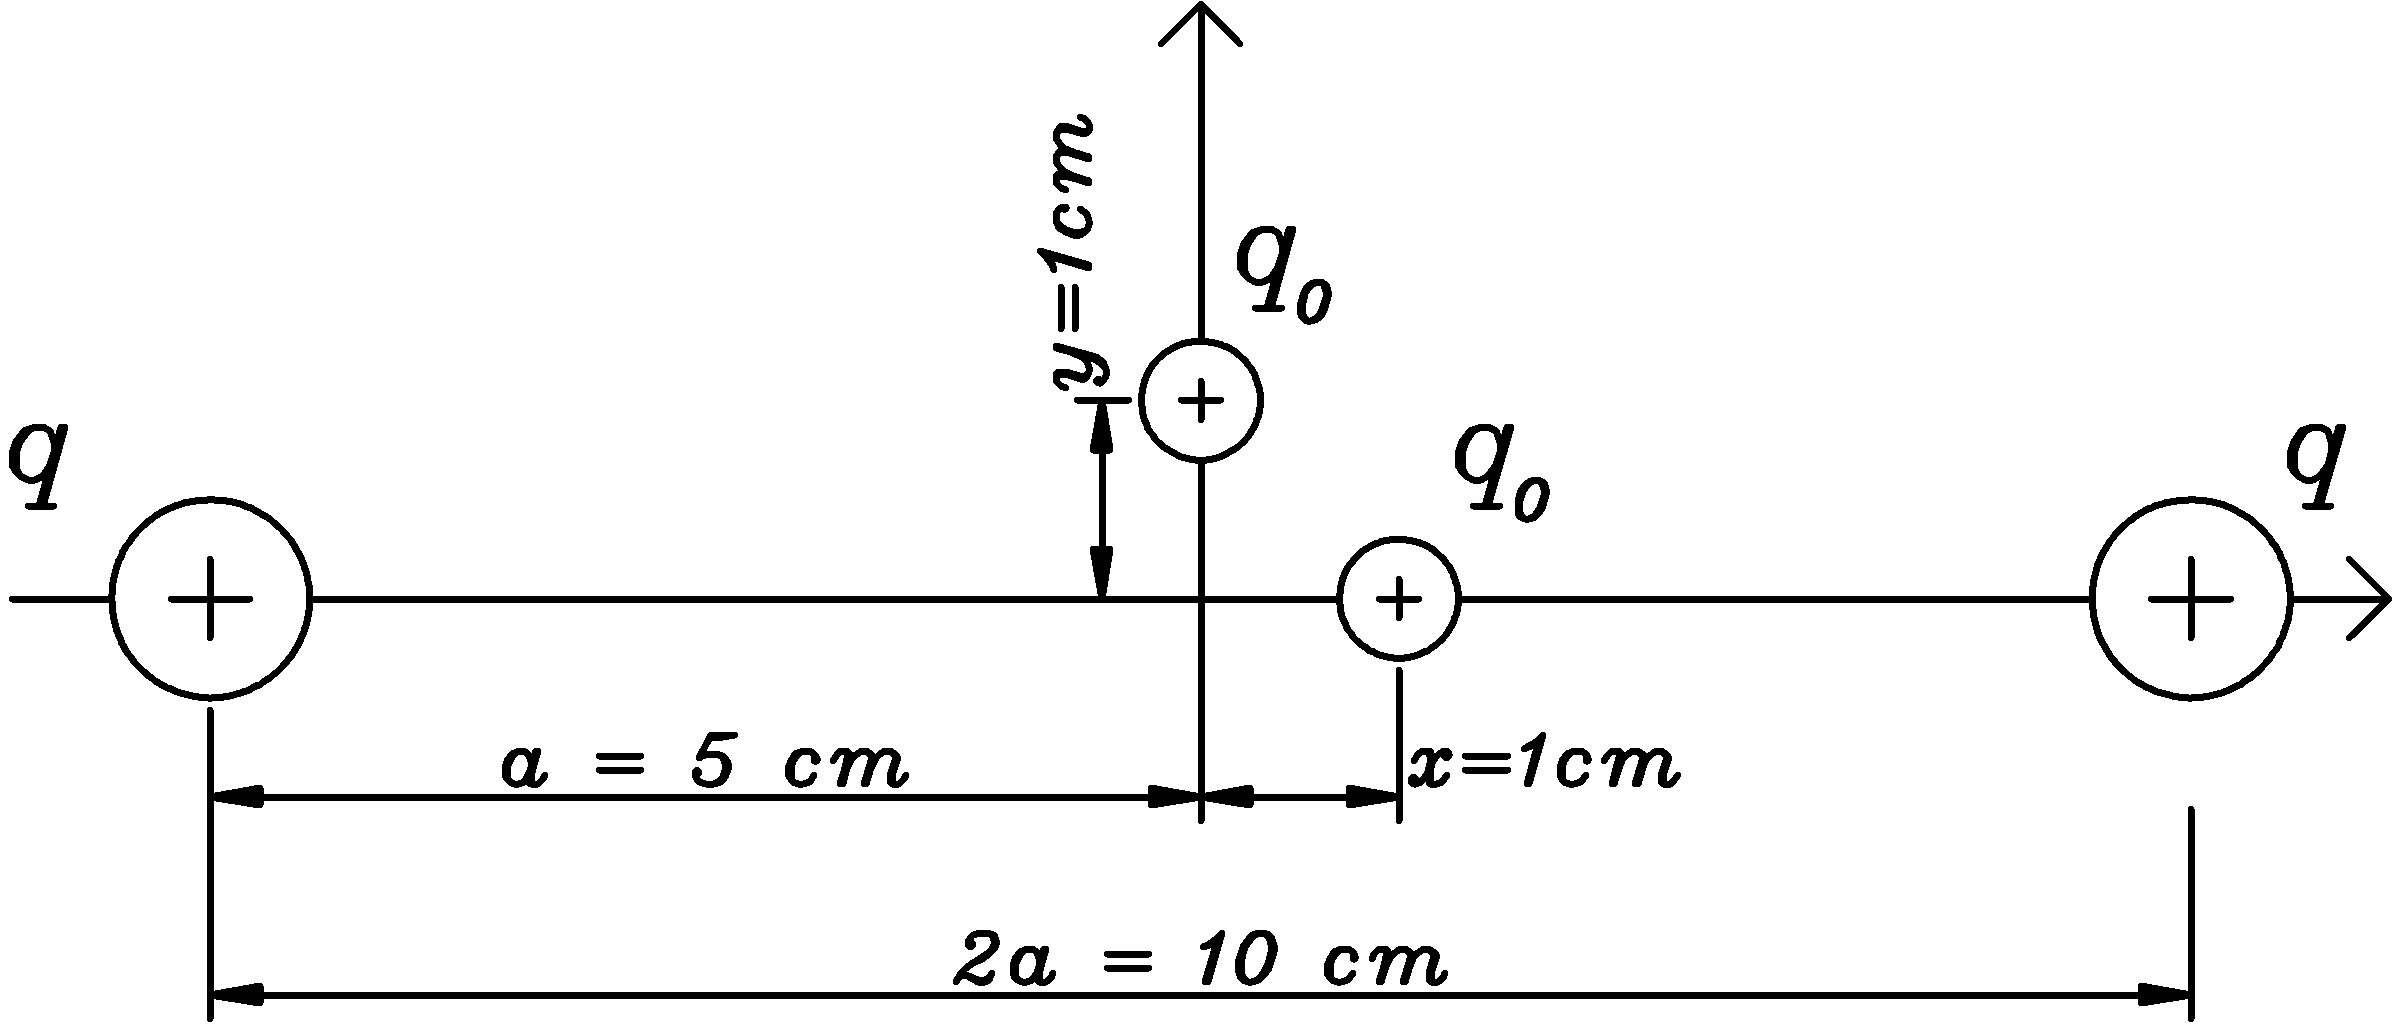
\includegraphics[width=10cm]{immagini/es_1-3.png} \centering
    \end{align*}
    Calcolare: 
    \begin{enumerate}
        \item la forza $F_x$ su una carica $q_0 = 10^{–10} C$ posta a distanza $x = 1 cm$ dal centro $O$
        \newline
        \textbf{Risoluzione}: Si calcolano le forze usando la legge di Coulomb, sapendo che la carica $q_0$ si trova ad $a + 1cm$ da $q_s$ ed a $a - 1cm$ da $q_d$, la risultante della forza su $q_0$ sarà la somma vettoriale delle forze $F_s$ tra $q_s$ e $q_0$ (orientata lungo il vettore $\vec{u_x}$), e $F_d$, tra $q_d$ e $q_0$ (orientata lungo il vettore $\vec{-u_x})$. Quindi
        \begin{align*}
            F_s & = \frac{1}{4 \pi \epsilon_0}\frac{q q_{0}}{(a + x)^2} \cdot \vec{u_x} \\
            F_d & = \frac{1}{4 \pi \epsilon_0}\frac{q q_{0}}{(a - x)^2} \cdot \vec{-u_x} \\
            F_x & = F_s + F_d = \frac{q q_{d}}{4 \pi \epsilon_0} \left( \frac{1}{(a + x)^2} \frac{1}{(a - x)^2} \right) = -6.53 \cdot 10^{-5} \vec{u_x} N
        \end{align*}
        \item la forza $F_y$ sulla stessa carica posta a distanza $y = 1 cm$ dal centro lungo l’asse delle due cariche.
        \newline
        \textbf{Risoluzione}: Si calcolano le componenti delle forze lungo l'asse $x$ e l'asse $y$. 
        \newline
        Lungo l'asse delle $x$ $q_1$ è equidistante da $q_d$ e $q_s$, Dunque $F_dx$ ed $F_sx$ saranno uguali in modulo ed opposte in verso, da qui ho
        \begin{align*}
            d_s = d_d \Rightarrow F_s = -F_d \Rightarrow F_s + F_d = 0
        \end{align*}
        Lungo l'asse delle $y$ $q_1$ è equidistante da $q_d$ e $q_s$, Dunque $F_dy$ ed $F_sy$ saranno uguali in verso ed in modulo. Inoltre la distanza $d$ sarà ottenuta tramite il teorema di Pitagora. Da qui
        \begin{align*}
            & d = \sqrt{a^2 + y^2} \\
            & d_s = d_d \Rightarrow F_s = F_d \Rightarrow F_s + F_d = 2F = 2 \cdot \frac{1}{4 \pi \epsilon_0}\frac{q q_{1}}{d^2} = 1.84 \cdot 10^{-5} N
        \end{align*}
    \end{enumerate}

    % 1.4
    \item Tre cariche $q_1 = 4 \cdot 10^{–8} C$, $q_2 = –2 \cdot 10^{–8} C$ e $q_3 = 6 \cdot 10^{–8} C$ sono allineate lungo l’asse $x$ in quest’ordine: la distanza tra $q_1$ e $q_2$ è uguale a quella tra $q_2$ e $q_3$ e vale $d = 50 cm$. Calcolare la forza $F_i$ esercitata su ciascuna carica dalle altre due.
    \newline
    \textbf{Risoluzione}: Calcolo il modulo delle interazioni fra le tre cariche e poi le sommo opportunamente (se la forza è $F$)
    \begin{align*}
        & F_{12} = \frac{1}{4 \pi \epsilon_0}\frac{q_{1}q_{2}}{d^2} = - 2.876 \cdot 10^{-5}N \\
        & F_{23} = \frac{1}{4 \pi \epsilon_0}\frac{q_{2}q_{3}}{(2d)^2} = -4.314 \cdot 10^{-5}N \\
        & F_{13} = \frac{1}{4 \pi \epsilon_0}\frac{q_{1}q_{3}}{d^2} = 8.628 \cdot 10^{-5}N \\
    \end{align*}
    Dunque le forze che agiranno sulle cariche saranno
    \begin{align*}
        & F_{q_1} = F_{12} (\vec{u_x}) + F_{13} (\vec{-u_x}) = - F_{12} - F_{13} = - 5.752 \cdot 10^{-5}N \vec{u_x} \\
        & F_{q_2} = F_{12} (\vec{-u_x}) + F_{23} (\vec{u_x}) = F_{12} - F_{23} = 1.438 \cdot 10^{-5}N \vec{u_x} \\
        & F_{q_3} = F_{13} (\vec{u_x}) + F_{23} (\vec{-u_x}) = F_{13} - F_{23} = 4.314 \cdot 10^{-5}N \vec{u_x} 
    \end{align*}
    
    % 1.5
    \item Tre cariche $q_1 = –4 \cdot 10^{–8} C$, $q_2 = –3 \cdot 10^{–8} C$ e $q_3 = 2 \cdot 10^{–8} C$ sono poste sui vertici di un triangolo equilatero di lato $l = 60 cm$. Calcolare la forza $F$ esercitata da $q_1$ e $q_2$ su $q_3$.
    \begin{align*}
        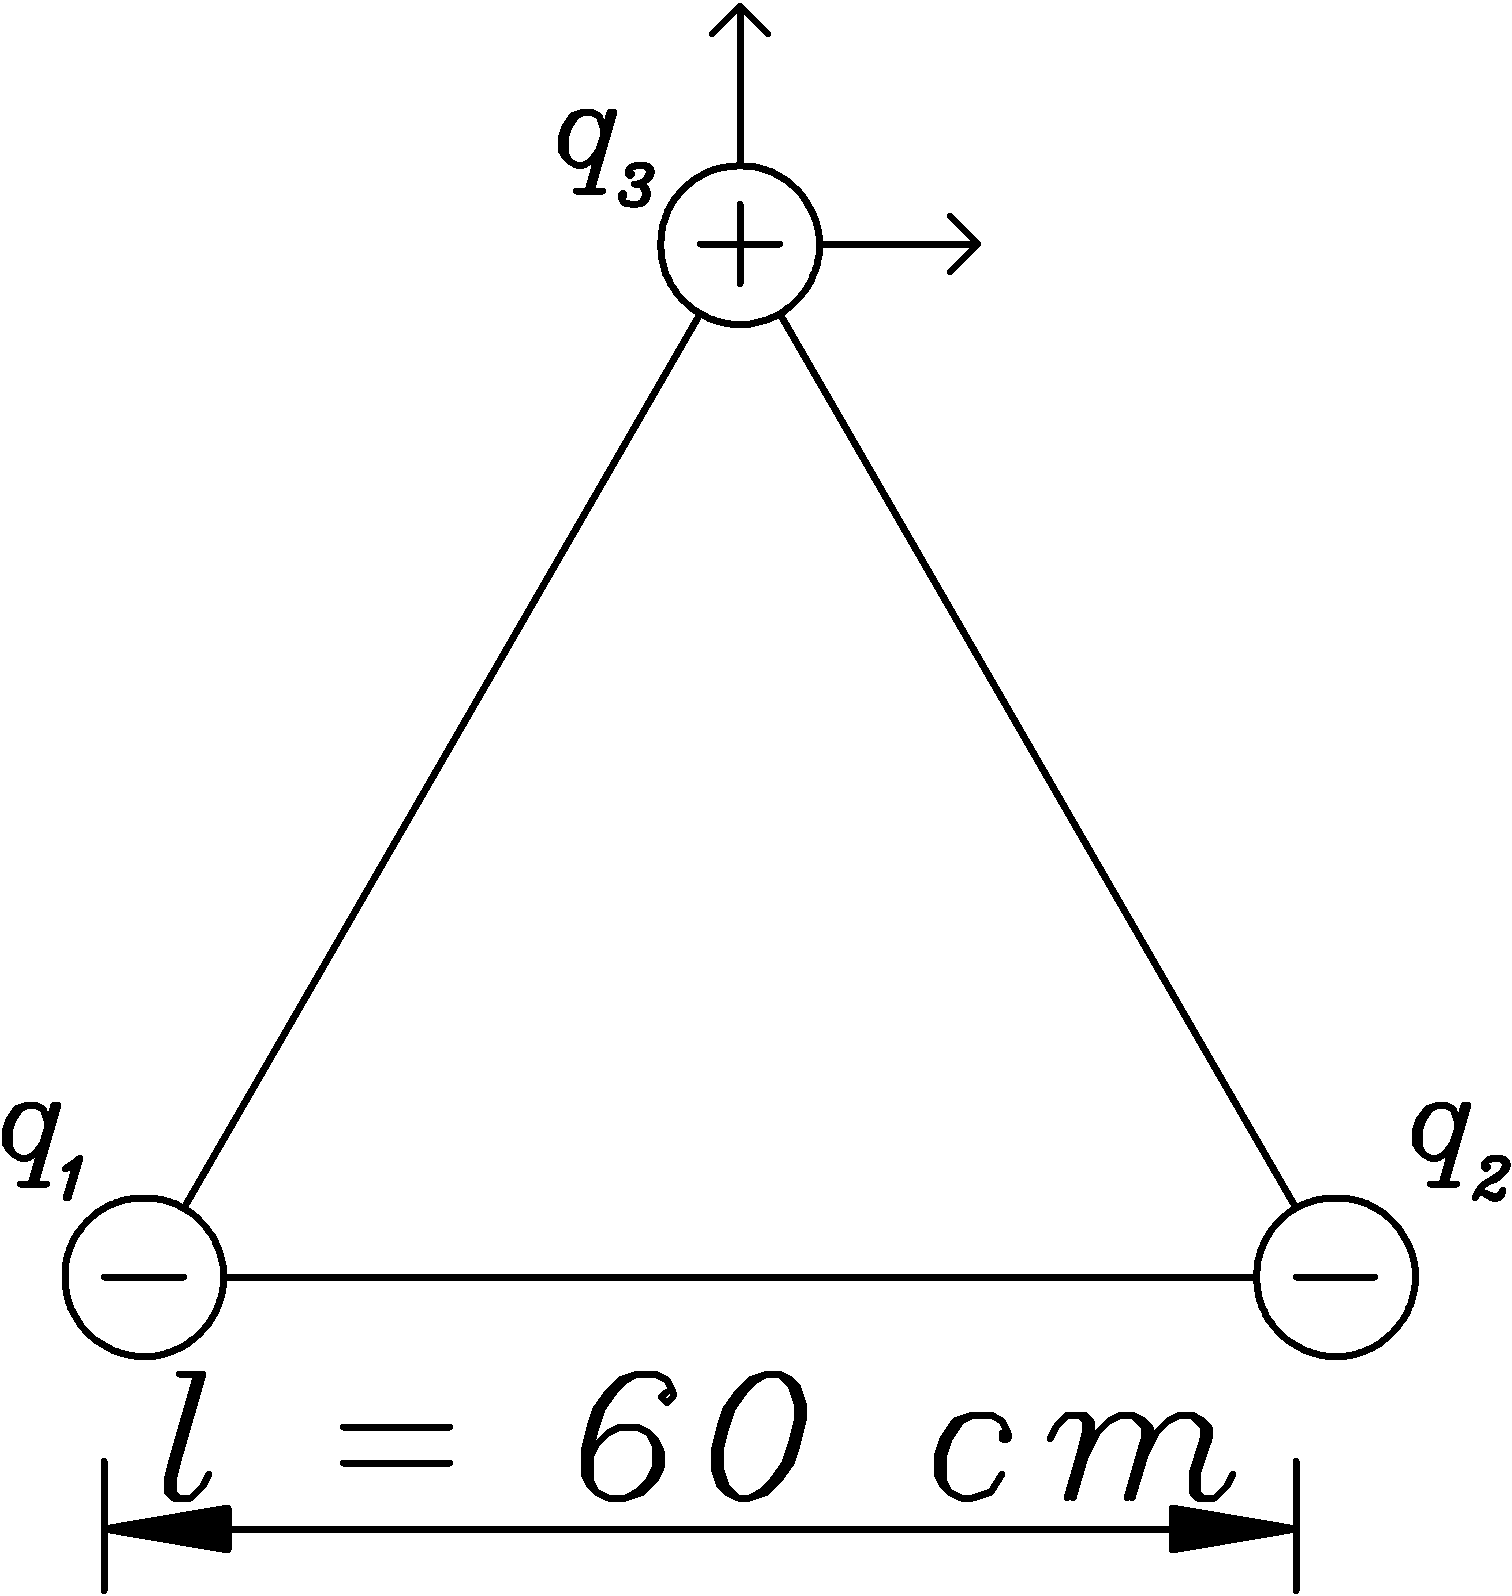
\includegraphics[width=4cm]{immagini/es_1-5.png} \centering
    \end{align*}
    \textbf{Risoluzione}: Dati i segni ed i valori delle cariche possiamo intuire che il verso lungo $x$ ed $y$ sarà negativo. Iniziamo calcolando i modulo delle forze $F_{13}$ ed $F_{23}$. Quindi otterremo le proiezioni lungo $x$ usando il coseno e lungo $y$ usando il seno. Raggruppando si ottiene
    \begin{align*}
        F_x &= \frac{1}{4 \pi \epsilon_0} \cdot \frac{q_1 q_3}{d^2} \cos(60°) - \frac{1}{4 \pi \epsilon_0} \cdot \frac{q_2 q_3}{d^2} \cos(60°) \\
            &= \frac{q_3 \cdot \cos(60°)}{4 \pi \epsilon_0 d^2}(q_1 - q_2) = -0.25 \cdot 10^{-5}N \\
        F_y &= \frac{1}{4 \pi \epsilon_0} \cdot \frac{q_1 q_3}{d^2} \sin(60°) - \frac{1}{4 \pi \epsilon_0} \cdot \frac{q_2 q_3}{d^2} \sin(60°) \\
            &= \frac{q_3 \cdot \sin(60°)}{4 \pi \epsilon_0 d^2}(q_1 + q_2) = -3.03 \cdot 10^{-5}N
    \end{align*}

    % 1.6 
    \item Quattro cariche uguali $q_i = q = 2 \cdot 10^{–8} C$ sono poste sui vertici di un rettangolo di lati $a = 10 cm$ e $b = 20 cm$. Calcolare la forza $F$ esercitata dalle altre tre cariche su $q_4$.
    \begin{align*}
        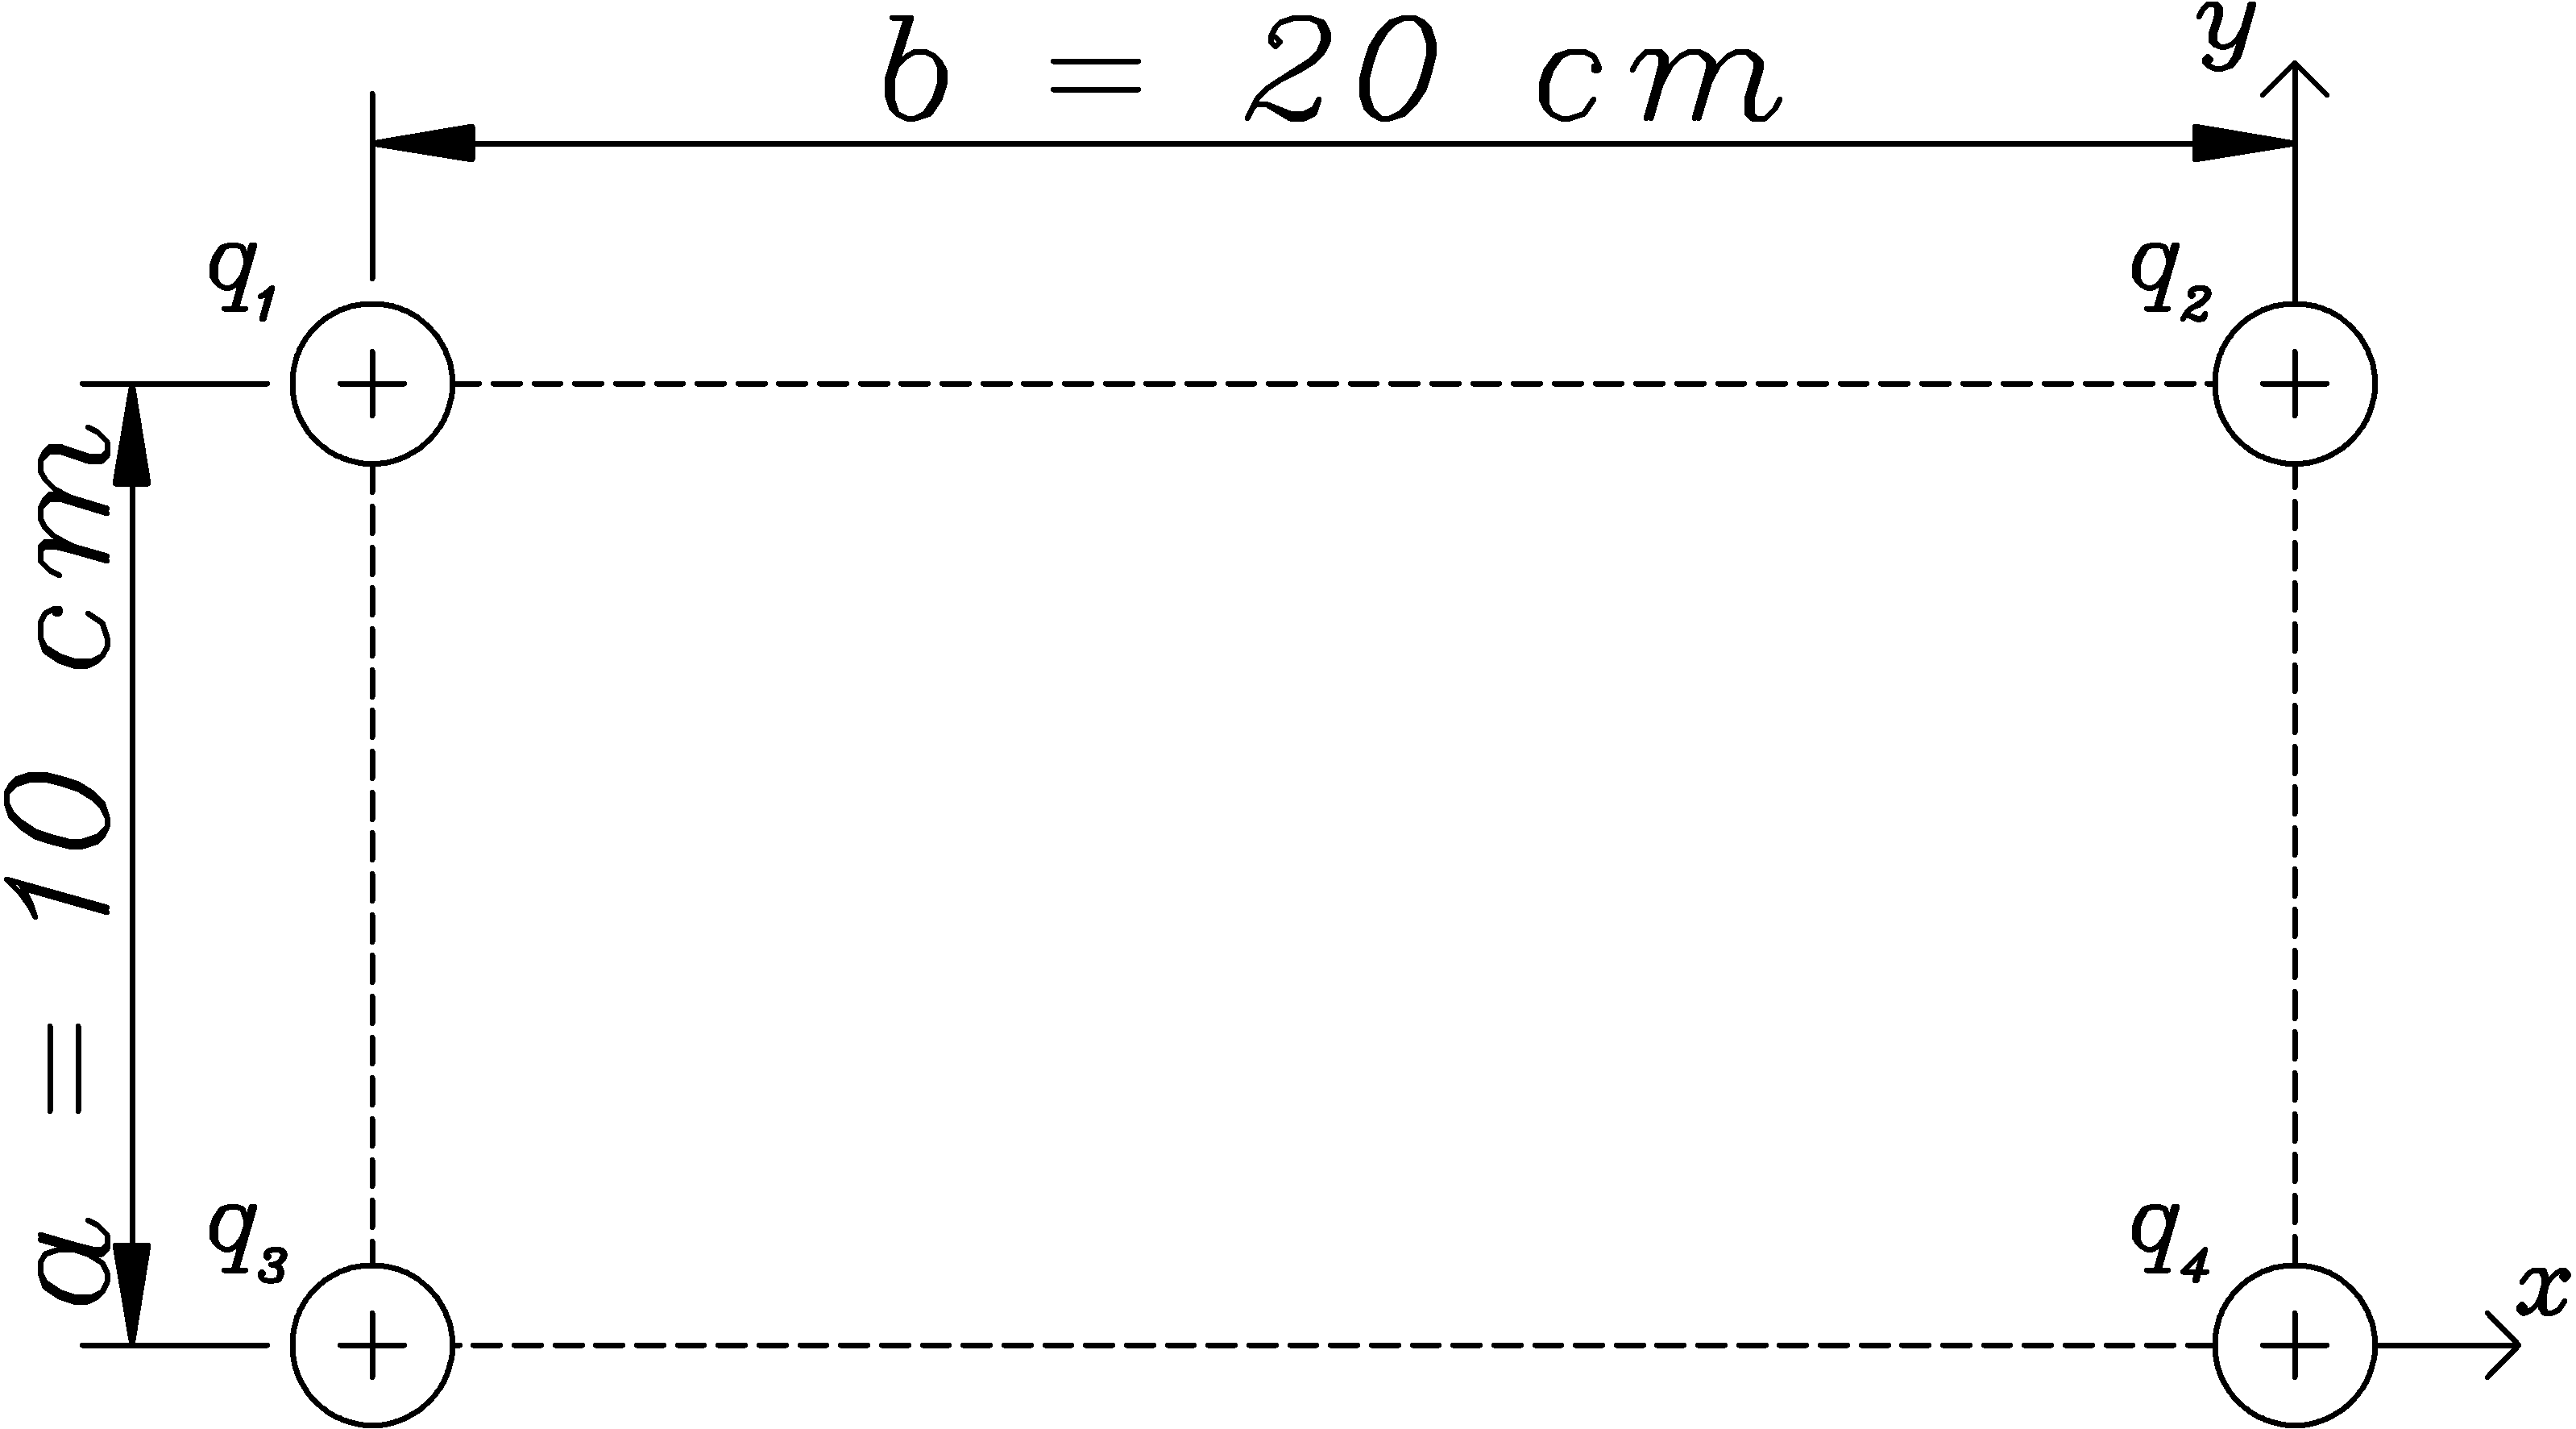
\includegraphics[width=7cm]{immagini/es_1-6.png} \centering
    \end{align*}
    \textbf{Risoluzione}: Date le distanze delle cariche dall'origine (centrata nella carica $q_4$), con la legge di Coulomb si possono ricavare i moduli delle forze, ricordando che sono orientate:
    \begin{enumerate}
        \item La forza tra $q_2$ e $q_4$ è orientata in direzione dell'asse $y$ ed in verso negativo (cioè lungo il vettore $\vec{-u_y}$).
        \item La forza tra $q_3$ e $q_4$ è orientata in direzione dell'asse $x$ ed in verso positivo (cioè lungo il vettore $\vec{u_x}$).
        \item La forza tra $q_1$ e $q_4$ è orientata in diagonale lungo il vettore $(\alpha \vec{u_x}, \beta \vec{-u_y})$ con $\alpha$, $\beta$ proiezioni della forza $F_{14}$ sugli assi cartesiani.
    \end{enumerate}
    Quindi procedendo al calcolo delle forze abbiamo che:
    \begin{align*}
        & d_{14} = \sqrt{a^2 + b^2} = 0.22 m \\
        & F_{14} = \frac{1}{4 \pi \epsilon_0}\frac{q_{1}q_{4}}{a^2 + b^2} = valore \\
        & d_{24} = a = 0.1 m \\
        & F_{24} = \frac{1}{4 \pi \epsilon_0}\frac{q_{2}q_{4}}{a^2} = valore \vec{-u_y} \\
        & d_{34} = b = 0.2 m \\
        & F_{34} = \frac{1}{4 \pi \epsilon_0}\frac{q_{3}q_{4}}{b^2} = valore \vec{u_x}
    \end{align*}
    Le proiezioni di $F_{14}$ sugli assi si potrebbero ottenere calcolando l'angolo $ \gamma = \arctan \left( \frac{-a}{b} \right)$ e poi proiettarlo usando le funzioni trigonometriche. 
    Tuttavia ricordandosi che:
    \begin{align*}
        & \sin(\gamma) = \frac{a}{d_{14}} \\
        & \cos(\gamma) = \frac{b}{d_{14}}
    \end{align*}
    otteniamo che le componenti di $F_{14}$ sono 
    \begin{align*}
        & F_{14}  \vec{ u_x} = \frac{1}{4 \pi \epsilon_0}\frac{q_{1}q_{4}}{a^2 + b^2} \cdot \frac{b}{\sqrt{a^2 + b^2}} = \frac{q_{1}q_{4}}{4 \pi \epsilon_0}\frac{b}{(a^2 + b^2)^{\frac{3}{2}}} = valore \\
        & F_{14}  \vec{-u_y} = \frac{1}{4 \pi \epsilon_0}\frac{q_{1}q_{4}}{a^2 + b^2} \cdot \frac{a}{\sqrt{a^2 + b^2}} = \frac{q_{1}q_{4}}{4 \pi \epsilon_0}\frac{a}{(a^2 + b^2)^{\frac{3}{2}}} = valore    
    \end{align*}
    Si sommano quindi le componenti per verso (sono concordi quando lungo gli stessi assi, quindi non bisognerà cambiare segno a nessun modulo).
    \begin{align*}
        & F_{14}  \vec{ u_x} + F_{24} = valore \\
        & F_{14}  \vec{-u_y} + F_{34} = valore 
    \end{align*}

    % 1.7
    \item lorem ipsum dolor sit amat consecetur eit
    \begin{align*}
        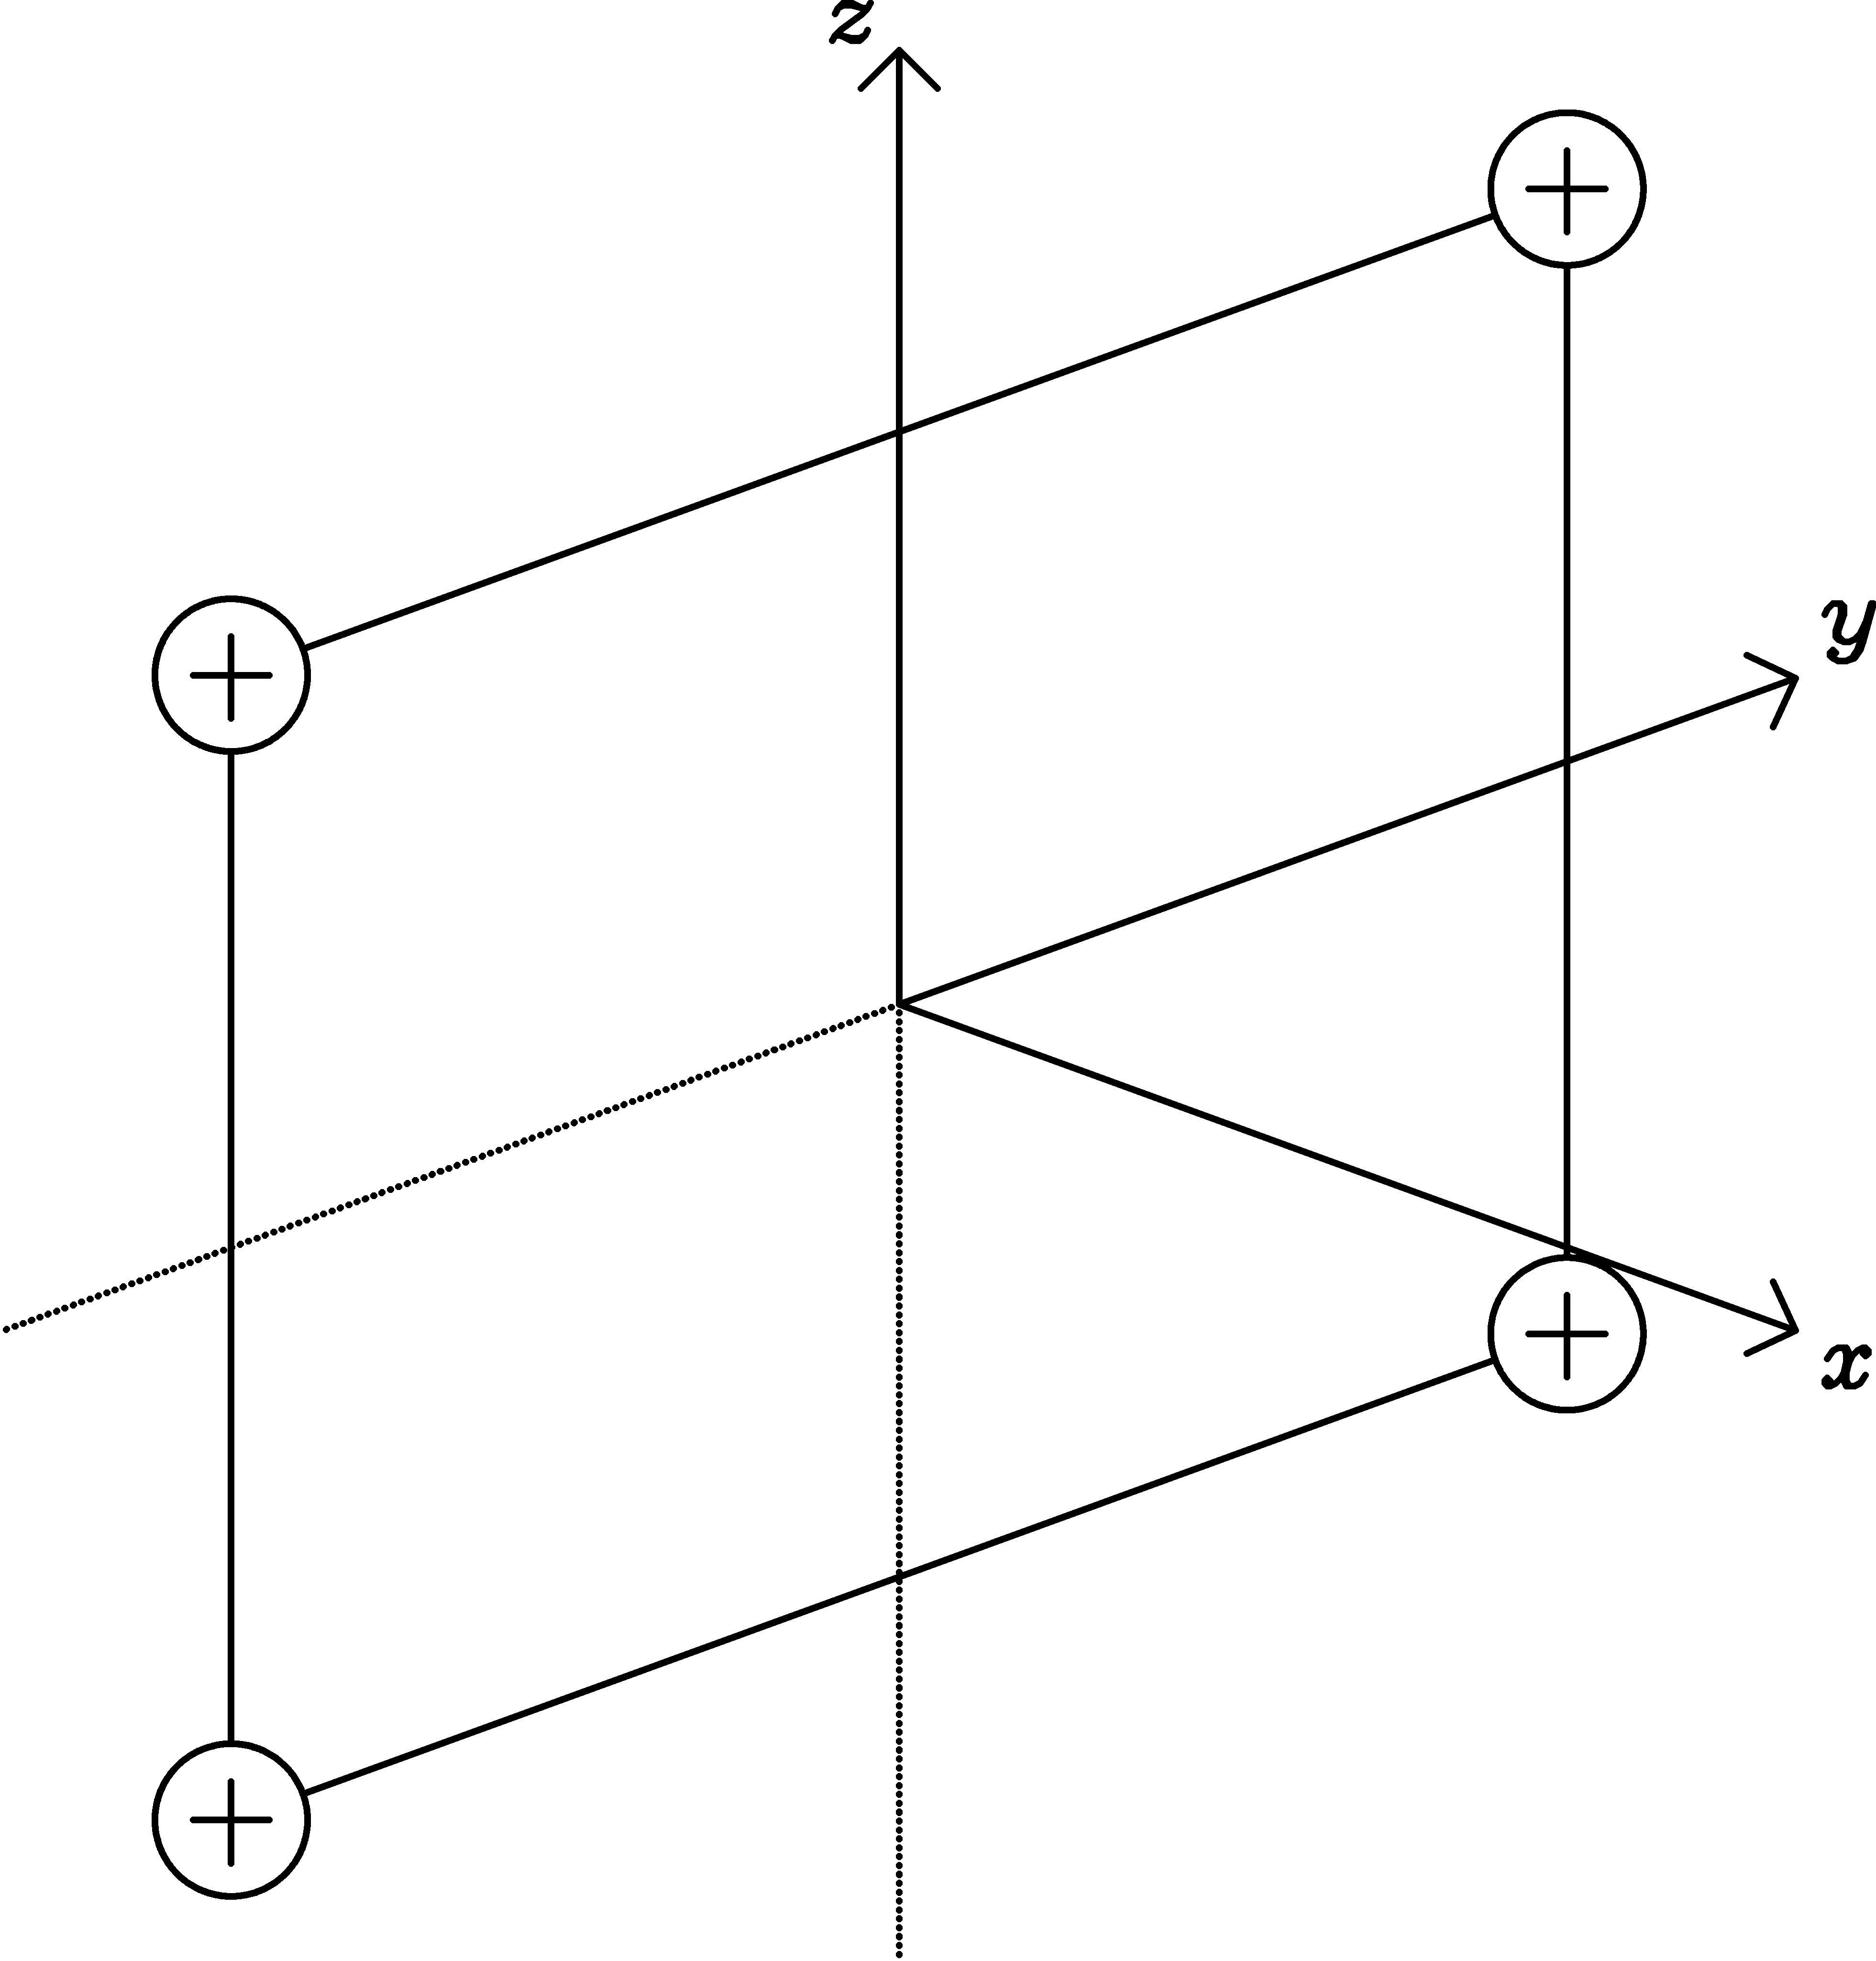
\includegraphics[width=7cm]{immagini/es_1-7.png} \centering
    \end{align*}
    \textbf{Risoluzione}:
   
    % 1.8
    \item 
\end{enumerate}

%----------------------------------------------------
\chapter{Lavoro elettrico e potenziale elettrostatico}



%----------------------------------------------------
\chapter{Legge di Gauss}


\begin{enumerate}
    %3.1
    \item Calcolare il flusso $\Phi(E)$ del campo elettrostatico $E = 2 \cdot 10^4  V/m$:
    \begin{enumerate}
        \item attraverso un quadrato di lato $l = 10 cm$, posto nel piano $yz$ 
        \newline
        \textbf{Risoluzione}: Usando le formule abbiamo che il flusso $\Phi(E)$:
        \begin{align*}
            \Phi (E) & = \int E u_x d \Sigma \\
                     & = E \int d \Sigma \\
                     & = E \cdot \Sigma
        \end{align*}
        Con $\Sigma$ superficie del quadrato con area pari a $l^2$. Da qui 
        \begin{align*}
            \Phi (E) = E \cdot l^2 = 2 \cdot 10^4 V/m \cdot 1 \cdot 10^{-2} m^2 = 2 \cdot 10^2 Vm
        \end{align*}
        \item attraverso lo stesso quadrato se la normale al quadrato forma un angolo $\alpha = 30^o$ con il campo $E$.
        \newline
        \textbf{Risoluzione}: Si prende il campo precedentemente calcolato e si calcola la sua proiezione sulla retta ortogonale al piano (quella su cui giace il flusso attraversante la superficie)
        \begin{align*}
            \Phi (E) = E \cdot \Sigma \cdot \cos(30^o) = 173.20 Vm
        \end{align*}
    \end{enumerate}
    %3.2
    \item Un campo elettrostatico uniforme $E = au_x + bu_y$ interseca una superficie piana di area $\Sigma$. Calcolare il flusso $\Phi(E)$ del campo $E$ attraverso la superficie $\Sigma$ nel caso in cui giacesse:
    \begin{enumerate}
        \item nel piano $xy$
        \newline
        \textbf{Risoluzione}: Essendo il piano lungo versori giacenti sugli assi $x$ ed $y$ ed essendo il flusso ortogonale alla superficie, e quindi lungo un versore sull'asse $z$, il flusso $\Phi (E)$ su questa superficie sarà nullo.

        \item nel piano $xz$
        \newline
        \textbf{Risoluzione}: In questo caso il flusso sarà orientato sull'asse $y$, dundue si azzererà la componente su $x$ lasciando il flusso pari a 
        \begin{align*}
            \Phi (E) = b \cdot \Sigma 
        \end{align*}

        \item nel piano $yz$
        \newline
        \textbf{Risoluzione}: Analogamente al caso precedente il flusso sarà orientato sull'asse $x$, quindi si azzererà la componente lungo $y$: da qui
        \begin{align*}
            \Phi (E) = a \cdot \Sigma 
        \end{align*}
    \end{enumerate}

    %3.3
    \item Calcolare il flusso $\Phi(E)$ del campo elettrostatico $E = 5 \cdot 10^5 xu_z V/m$ attraverso il quadrato di lato $a = 5 cm$, orientato con la normale concorde con $uz$.
    \begin{align*}
        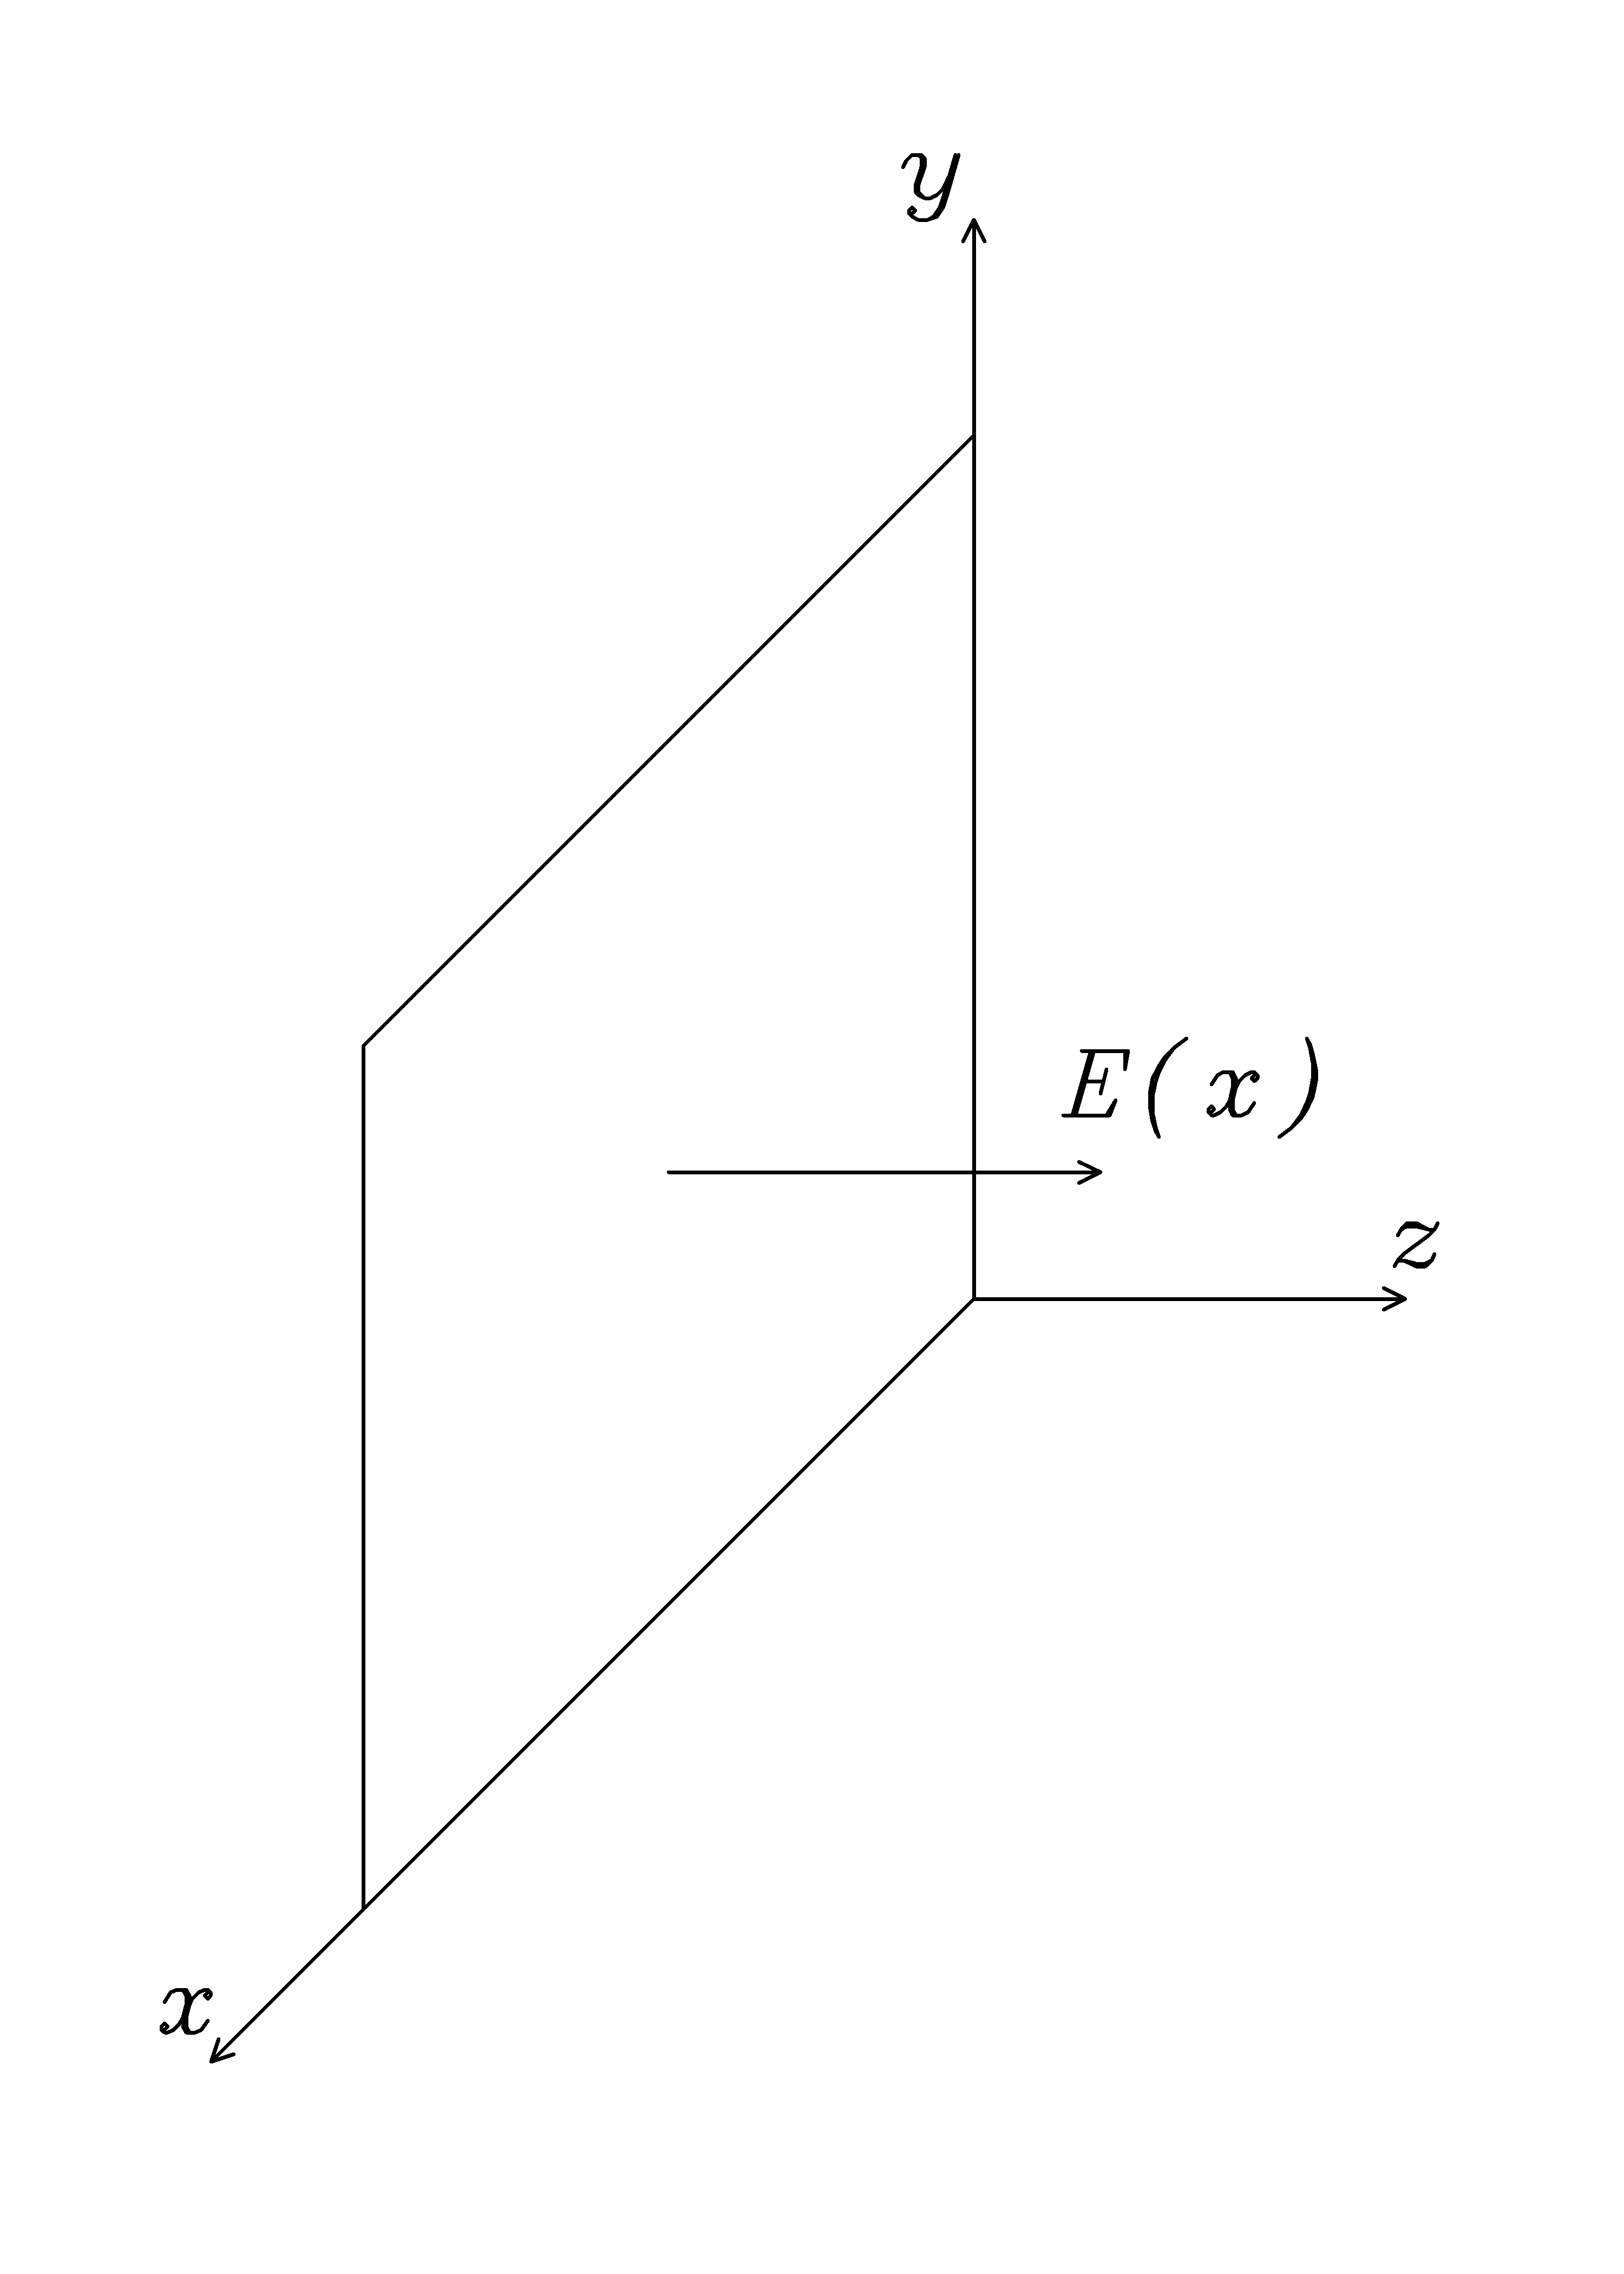
\includegraphics[width=7cm]{immagini/es_3-3.png} \centering
    \end{align*}
    \newline
    \textbf{Risoluzione}: Analogamente al primo caso calcoliamo $\Phi(E)$, ma il campo $E$ non è costante, quindi con un integrale ottengo
    \begin{align*}
        \Phi(E) & = E \cdot \Sigma \\
                & = \Sigma \int_{0}^{a}Edx  \\
                & = \int_{0}^{a} 5 \cdot 10^5 a x dx \\ 
                & = \left[5 \cdot 10^5 \frac{a \cdot x^2}{2} \right]_{0}^{a} \\
                & = 5 \cdot 10^5 \cdot \frac{a^3}{2} = 31.25 Vm
    \end{align*}
    \textbf{Domanda}: che fine ha fatto $\Sigma$?
    \newline
    Invece che portarla fuori e rischiare di trovare esponenti di troppo, considero la superficie come una retta ad altezza $a$ dall'asse $x$ (quindi $y = a$) ed integro.
    Essendo l'integrale di una retta parallela all'asse $x$ uguale all'area del rettangolo sotteso tra la retta e l'asse, ottengo la superficie che cercavo.
    \newline 
    \textbf{Domanda}: come posso separare le due cose senza trovarmi un $a^4$ indesiderato nella formula finale?
    \newline
    Non essendo il campo costante non posso integrare area e campo in due volte diverse, in quanto sono legati l'uno all'altro. 
    Per intenderci, prendendo un infinitesiomo del campo molto vicino all'origine, questi avrà effetto su una piccola superficie del rettangolo, e lo stesso vale per un infinitesimo molto lontano:
    sarebbe quindi sbagliato pensare che il campo agisce uniformemente sulla superficie.

    % 3.4
    \item Con riferimento alla figura, il campo elettrostatico $E$ varia con la legge $E = (5 + 4x^2) \cdot 10^5 u_x V/m$ con $x$ espresso in metri. Calcolare, dato il parallelepipedo di lati $a = 10 cm$, $b = 15 cm$, $c = 20 cm$: 
    \begin{enumerate}
        \item il flusso $\Phi (E)$ attraverso il parallelepipedo
        \newline 
        \textbf{Risoluzione}: Il flusso è diretto lungo l'asse $x$ dunque tutte le facce non parallele al piano $yz$ avranno di conseguenza flusso $\Phi(E) = 0$. Si procede dunque al calcolo:
        \begin{align*}
            \begin{cases}
                x=0 \\
                \Phi(E) = ab \cdot 5 \cdot 10^5 V/m = 7.5 \cdot 10^3 Vm
            \end{cases}
            \begin{cases}
                x = c\\
                \Phi(E) = ab \cdot (5 + 4c^2) \cdot 10^5 V/m = 7.74 \cdot 10^3 Vm
             \end{cases}
        \end{align*}
        \begin{align*}
            \Phi(E) = ab[E(c) - E(0)] = 4 \cdot 10^5 abc^2 Vm = 240Vm
        \end{align*}

        \item la carica $q$ contenuta all’interno di tale parallelepipedo
        \newline 
        \textbf{Risoluzione}: Conoscendo la formula $\Phi(E) = \frac{q}{\epsilon_0}$ ricaviamo $q$
        \begin{align*}
            q = \epsilon_0 \Phi(E) = 2.13 \cdot 10^{-9} C
        \end{align*}
    \end{enumerate}
   
    %3.5
    \item Il campo elettrostatico in una certa regione dello spazio è dato da $E = (5xu_x - 4yu_y + 3zu_z) \cdot 10^5 V/m$. Calcolare, data la superficie  mostrata in figura di lati $a = 10 cm$, $b = 15 cm$ e $c = 20 cm$: 
    \begin{enumerate}
        \item il flusso $\Phi(E)$ attraverso la superficie chiusa
        \newline 
        \textbf{Risoluzione}: Usiamo la formula 
        \begin{align*}
            \Phi(E) & = \int \nabla \cdot E dt \\
                    & = \nabla E \cdot abc \\
                    & = 1.2 \cdot 10^3 Vm
        \end{align*}

        \item la carica $q$ presente all’interno della superficie
        \newline 
        \textbf{Risoluzione}: Come nel punto 4.b si usa la formula 
        \begin{align*}
            q = \epsilon_0 \Phi(E) = 1.06 \cdot 10^{-8} C
        \end{align*}

        \item la sua densità di carica $\rho$ nell’ipotesi che essa sia costante all’interno della superficie stessa
        \newline 
        \textbf{Risoluzione}: Con le formule inverse abbiamo che:
        \begin{align*}
            & \Phi(E) = \nabla E \cdot abc \Rightarrow \\
            & \begin{cases}
                \nabla E = \frac{\Phi(E)}{abc} 
                \nabla E = \frac{1}{\epsilon_0} \cdot \rho 
            \end{cases} \\
            & \Rightarrow \rho = \epsilon_0 \frac{\Phi(E)}{abc} = 3.54 \cdot 10^{-6} C/m^3
        \end{align*}
    \end{enumerate}
    
    % 3.6
    \item Una carica $q_0$ è posta sull’asse di un disco uniformemente carico con densità superficiale $\sigma = –5 \cdot 10^{–8} C/m^2$. Il flusso del campo della carica $q_0$ attraverso la superficie del disco vale $\Phi(E) = 4 \cdot 10^3 Vm$. Calcolare la forza $F$ esercitata dal disco su $q_0$.
    \begin{align*}
        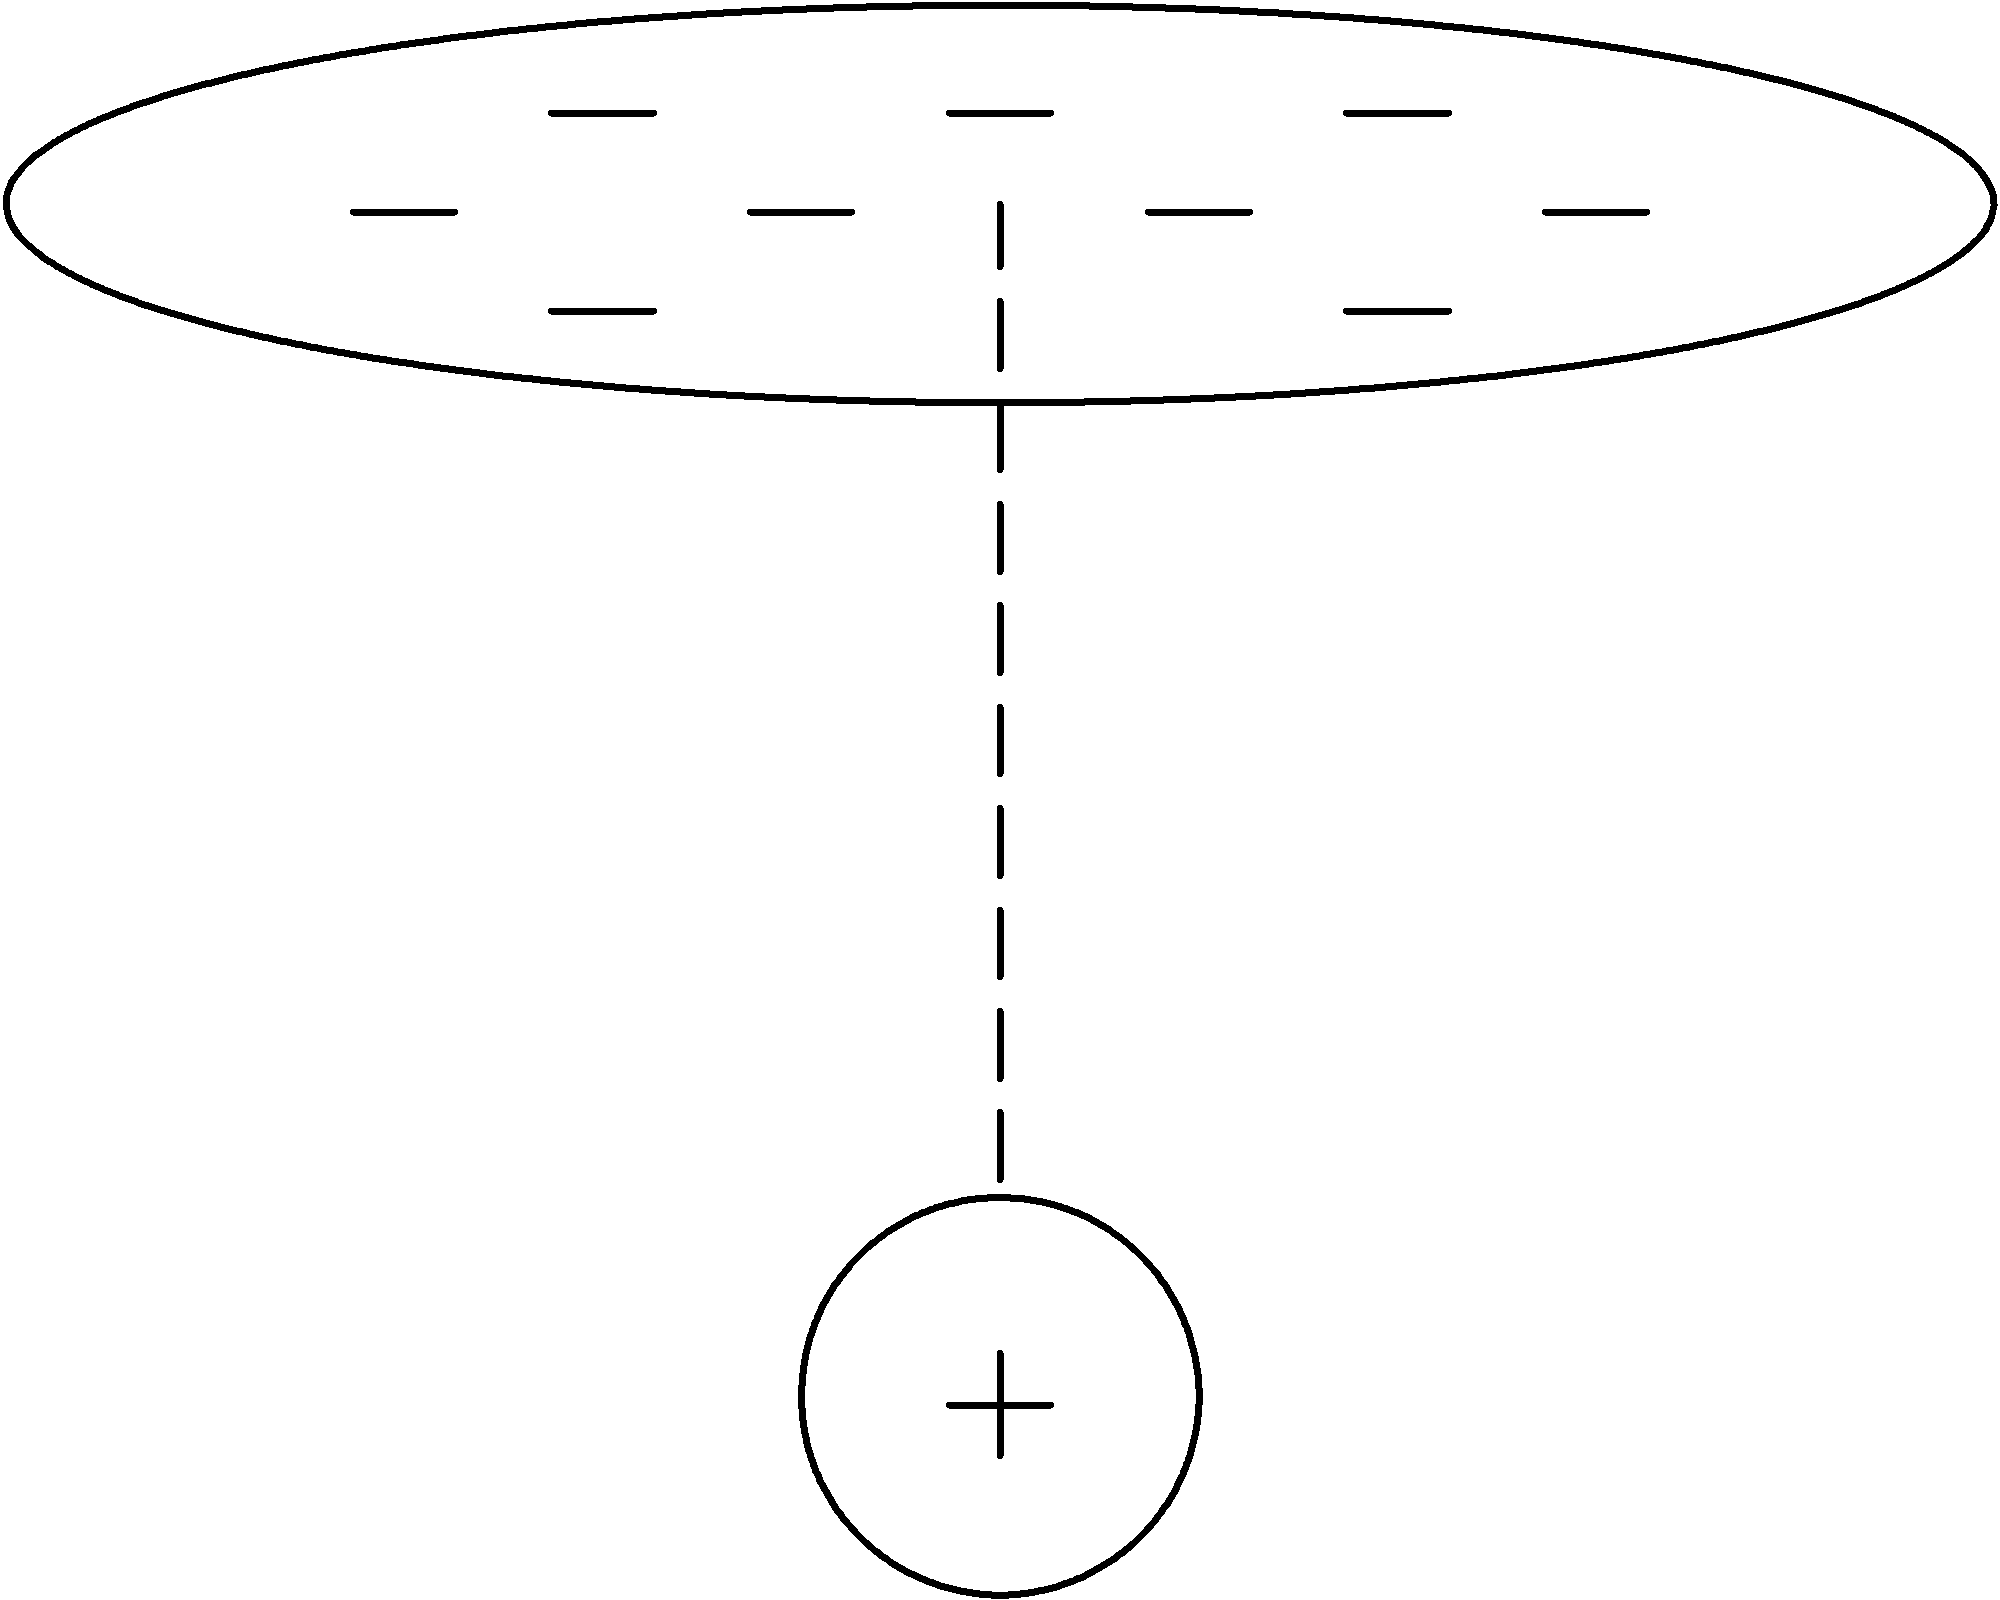
\includegraphics[width=7cm]{immagini/es_3-6.png} \centering
    \end{align*}
    \newline 
    \textbf{Risoluzione}: Si ricava da due formule e passando per l'angolo solido:
    \begin{align*}
        &\begin{cases}
            \Omega = 2 \pi (1- cos(\theta)) \\
            \Phi(E) = \int_{\Sigma} E u_n d\Sigma = \frac{q}{4 \pi \epsilon_0} \int_{\Omega}d\Omega = \frac{q}{4 \pi \epsilon_0} \Omega
        \end{cases} \\
        & \Rightarrow \Phi(E) = \frac{q}{2 \epsilon_0}(1-cos(\theta))
    \end{align*}

    % 3.7
    \item Con riferimento alla figura, per il flusso del campo elettrostatico prodotto dal sistema di cariche sono dati i seguenti valori: $\Phi_{\Sigma1}(E) = –1.13 \cdot 10^3 Vm$, $\Phi{\Sigma2}(E) = \Phi{\Sigma3}(E) = 0$ e $\Phi{\Sigma4}(E) = 4.514 \cdot 10^3 Vm$. Calcolare $q_1$, $q_2$, $q_3$ e $q_4$.
    \newline 
    \textbf{Risoluzione}: Sapendo che $$\Phi(E) = \frac{1}{\epsilon_0}\Sigma_{i=1}^{n}q_i$$ ricavo che:
    \begin{align*}
        & q_1 = \epsilon_0 \Phi_{\Sigma1}(E) \\
        & q_1 + q_4 = \epsilon_0 \Phi_{\Sigma2}(E) = 0 \Rightarrow q_4 = -q_1 \\
        & q_3 + q_4 = \epsilon_0 \Phi_{\Sigma3}(E) = 0 \Rightarrow q_3 = -q_4 = q_1 \\
        & q_2 + q_3 = \epsilon_0 \Phi_{\Sigma4}(E) \Rightarrow q_2 = \epsilon_0 \Phi_{\Sigma4}(E) - q_3
    \end{align*}
    Calcolando ottengo che 
    \begin{align*}
        q_1 & = -1 \cdot 10^{-8}C \\
        q_2 & = -3 \cdot 10^{-8}C \\
        q_3 & = -1 \cdot 10^{-8}C \\
        q_4 & =  1 \cdot 10^{-8}C
    \end{align*}
    
    % 3.8

    \item Con riferimento alla figura, $q1 = q = –10–8 C$ e il flusso del campo elettrostatico $E$ attraverso le superfici tratteggiate risulta: $\Phi_{\Sigma1}(E) = \Phi_{\Sigma2}(E) = 0$, $\Phi_{\Sigma3}(E) = 2.26 \cdot 10^3 Vm$. Calcolare $q_2$, $q_3$ e $q_4$.
    \newline 
    \textbf{Risoluzione}: Identica all'esercizio precedente.

\end{enumerate}



%----------------------------------------------------
\chapter{Conduttori ed energia elettrostatica}

\begin{enumerate}

    %4.1
    \item Una sfera di rame di raggio $R = 10cm$ possiede una carica $q=10^-8 C$. Determinare ogni quanti atomi della sfera manca un elettrone. Per il rame: $mmol=63.55 g/mol, \rho = 8.96 \cdot 10^3 kg/m^3$\newline
    \textbf{Risoluzione}: si calcola prima il numero di elettroni che serve per avere la carica $q$ ($N^oe^-$), si calcolano quindi gli atomi in una sfera di rame di raggio $r = 10cm$ ($n^oCu$), quindi si fa il rapporto $n^oCu/n^oe^-$.
        \begin{align*}
            & n^o e^- =\frac{q}{e}=\frac{10^-8 C}{1.602 \cdot 10^-19 C} = 6.242 \cdot 10^{10} \\
            & vol \Sigma = \frac{4}{3} r^3 \pi = \frac{4}{3} \cdot 0.1m^3 \pi= 4.19 \cdot 10^{-3} m^3 =  4.19 \cdot 10^{6} cm^3 \\
            & mol Cu = \frac{vol\Sigma \cdot \rho }{mmolCu} = \frac{ 4.19 \cdot 10^{6}cm^3 \cdot 8.96 g/cm^3}{63.55 g/mol} = 5.9 \cdot 10^5mol \\
            & n^o Cu =  molCu * n^o Avogadro = 5.9 \cdot 10^5 mol \cdot 6.022 \cdot 10^{23} 1/mol = 3.5 \cdot 10^{26} \\
            & Cu/e^- = \frac{n^o Cu}{n^o e^-} = \frac{3.5 \cdot 10^{29}}{6.242 \cdot 10^{10}} = 5.6 \cdot 10^{18} \\
            & RICONTROLLA-I-CONTI
        \end{align*}

    %4.2
    \item La rigidità dielettrica dell'aria secca è $E_s=3\cdot 10^6V/m$. Calcolare:
        \begin{enumerate}
            \item La massima carica  $q_{max}$ che può essere depositata su una sfera conduttrice di raggio $r=10cm$ \newline
            \textbf{Risoluzione}: Il campo elettrostatico sulla superficie della sfera è uguale alla rigidità dielettrica dell'aria e si calcola come il rapporto fra la carica sulla superdicie della sfera e la superficie della sfera (DA RICONTROLLARE), quindi
                \begin{align*}
                    & E_s = \frac{q_{max}}{4\pi \epsilon_0 r^2}
                \end{align*}
                Da qui posso ricavare $q_{max}$ come
                \begin{align*}
                    & q_{max} = \frac{4 \pi \epsilon_0 r^2}{E_s} = 3.33 \cdot 10^{-6}C
                \end{align*}
            \item Il potenziale massimo $V_{max}$ assunto.\newline
            \textbf{Risoluzione}: Dato che la rigidità dielettrica è definita come il valore limite del campo elettrico, $V_{max}$ ed $E_s$ sono uguali, ergo
                \begin{equation*}
                    V_{max} = E_s = 3 \cdot 10^6V/m
                \end{equation*}
        \end{enumerate}

    %4.3
    \item In un giorno secco il campo elettrostatico vicino alla superficie terrestre è $E = 100V/m$ ed è diretto verso la Terra. Nell'ipotesi che E sia costante su tutta la superficie terrestre ($R_T=6360km$) calcolare quale sarebbe la carica $q$ presente sulla superficie terrestre, se non ci fossero altri effetti che in pratica tendono a farla diminuire apprezzabilmente. \newline
        \textbf{Risoluzione}:  data una sfera conduttrice isolata, uniformemente carica, il campo elettrostatico prodotto all'esterno vale
        \begin{equation*} 
            E=\frac{q}{4\pi\epsilon_0 r^2}
        \end{equation*}
        mentre il potenziale vale
        \begin{equation*} 
            V=\frac{q}{4\pi\epsilon_0 r}
        \end{equation*}
        valore assunto anche all'interno. Quindi la carica $q$ sarà uguale a 
        \begin{equation*}
            q=E \cdot 4\pi\epsilon_0 r^2=4.49\cdot 10^5C
        \end{equation*}

    %4.4
    \item Due sfere conduttrici $S_1$ ed $S_2$ di raggi rispettivamente $r_1$ ed $r_2$ sono poste nel vuoto ad una distanza $x$ tra i centri, molto grande rispetto ad $ r_1$ ed $r_2$. La sfera $S_1$, isolata, ha una carica $q_1$, mentre $S_2$ è mantenuta ad un potenziale $V_2$ rispetto all'infinito. Calcolare:
    \begin{enumerate}
        \item Il potenziale $V_1(x)$ della sfera $S_1$ \newline
        \textbf{Risoluzione}: 
        \item La carica $q_2(x)$ della sfera $S_2$ \newline
        \textbf{Risoluzione}: 
        \item La forza $F(x)$ tra le sfere in funzione della distanza $x$ \newline
        \textbf{Risoluzione}: 
    \end{enumerate}

    %4.5
    \item Una piccola sfera conduttrice di raggio $r_s=1mm$ è posta sull'asse di un disco di raggio $r_d=10cm$, uniformemente carico con densità $\sigma=10^{-11}C/m^2$; il centro della sferetta dista d=30cm dal centro del disco. La sferetta è collegata a terra da un sottile filo conduttore, così che il suo potenziale sia nullo. Calcolare la carica $q$ sulla sferetta. \newline
    \textbf{Risoluzione}: Si comincia calcolando il potenziale nel punto a distanza $d$ dal centro del disco sull'asse. Iniziamo la discesa nella follia considerando il disco come un'insieme di cirdonferenze, e che sommandole tutte otteniamo l'area del disco.
    Moltiplicando l'area del disco per la densità di carica otterremo la carica del disco, dunque:
    \begin{align*}
        q = \int_{0}^{r_d}\sigma \cdot 2 \pi r dr 
    \end{align*}
    Consideriamo la distanza tra il pundo e la circonferenza in cui abbiamo suddiviso il disco (che chiamerò distanza integrale $d_i$) come 
    \begin{align*}
        d_i = \sqrt{r^2+d^2}
    \end{align*}
    Mentre l'insieme delle distanze sarà il suo integrale per $r$ che va da $0$ a $r_d$. \newline
    Quindi calcoliamo il potenziale $V$ come:
    \begin{align*}
        V & = \frac{1}{4 \pi \epsilon_0} \cdot \frac{q}{d} \\
          & = \frac{1}{4 \pi \epsilon_0} \int_{0}^{r_d} \frac{\sigma \cdot 2 \pi r}{\sqrt{r^2 + d^2}}dr \\
          & = \frac{2 \pi \cdot \sigma}{2 \cdot 2 \pi \cdot \epsilon_0} \int_{0}^{r_d} \frac{r}{\sqrt{r^2 + d^2}}dr \\
          & = k \cdot \int \frac{f(x)}{g(x)}dx= \frac{f'(x)g(x) + f(x)g'(x)}{g^2(x)} \\
          & = \left[ \frac{\sigma}{2 \epsilon_0} \cdot \frac{\sqrt{r^2+d^2} + \frac{1}{2} r^2 \sqrt{r^2 + d^2}}{r^2 + d^2} \right]_{0}^{r_d}\\
          & = \left[ \frac{\left( 1 + \frac{r^2}{2}\right)}{\sqrt{r^2 + d^2}} \right]_{0}^{r_d} \\
          & = 8.9 \cdot 10^{-3}V
    \end{align*}
    Esiste inoltre un $V_i$ sulla sferetta tale che sono soddisfatte le equazioni
    \begin{align*}
        & V_d + V_i = 0 \\
        & V_i = \frac{q_i}{4 \pi \epsilon_0 r_i}
    \end{align*}
    Da qui ricaviamo facilmente che $q_i = -1 \cdot 10^{-15} C$

\end{enumerate}


%----------------------------------------------------

\tableofcontents
\end{document}